\chapter{Suppl\texorpdfstring{ementary}{.} material for Chap\texorpdfstring{ter}{.}
\getrefnumber{ch:Transcriptomics}}\label{ch:app-Transcriptomics}
\chaptermark{Supplementary material for Chapter \getrefnumber{ch:Transcriptomics}}

\begin{figure}[!htbp]
\centering
\begin{subfigure}[b]{0.60\textwidth}
\centering \includegraphics[width=\textwidth]%
{transcriptomics/UniqueExpression/Castle_1.pdf}
\caption{Castle}\label{fig:UniqueExprCastle}
\end{subfigure}%
~%
\begin{subfigure}[b]{0.60\textwidth}
\centering \includegraphics[width=\textwidth]%
{transcriptomics/UniqueExpression/Brawand_1.pdf}
\caption{Brawand}\label{fig:UniqueExprBrawand}
\end{subfigure}

\begin{subfigure}[b]{0.60\textwidth}
\centering \includegraphics[width=\textwidth]%
{transcriptomics/UniqueExpression/IBM_1.pdf}
\caption{IBM}\label{fig:UniqueExprIBM}
\end{subfigure}%
~%
\begin{subfigure}[b]{0.60\textwidth}
\centering \includegraphics[width=\textwidth]%
{transcriptomics/UniqueExpression/Uhlen_1.pdf}
\caption{Uhlen}\label{fig:UniqueExprUhlen}
\end{subfigure}

\begin{subfigure}[b]{0.95\textwidth}
\includegraphics[width=\textwidth]%
{transcriptomics/UniqueExpression/Gtex_1b.pdf}
\caption{Gtex}\label{fig:UniqueExprGtex}
\end{subfigure}
\caption{Number of protein-coding genes expressed per tissue}\label{fig:UniqExprPC1}
\end{figure}


\begin{figure}[!htbp]
\centering
\begin{subfigure}[b]{0.60\textwidth}
\centering \includegraphics[width=\textwidth]%
{transcriptomics/UniqueExpression/CastleBreadthP1.pdf}
\caption{Castle}\label{fig:breadthCastleP1}
\end{subfigure}%
~%
\begin{subfigure}[b]{0.60\textwidth}
\centering \includegraphics[width=\textwidth]%
{transcriptomics/UniqueExpression/BrawandBreadthP1.pdf}
\caption{Brawand}\label{fig:breadthBrawandP1}
\end{subfigure}%

\begin{subfigure}[b]{0.60\textwidth}
\centering \includegraphics[width=\textwidth]%
{transcriptomics/UniqueExpression/IBMBreadthP1.pdf}
\caption{IBM}\label{fig:breadthIBMP1}
\end{subfigure}%
~%
\begin{subfigure}[b]{0.60\textwidth}
\centering \includegraphics[width=\textwidth]%
{transcriptomics/UniqueExpression/UhlenBreadthP1.pdf}
\caption{Uhlen}\label{fig:breadthUhlenP1}
\end{subfigure}%

\begin{subfigure}[b]{0.95\textwidth}
\includegraphics[width=\textwidth]%
{transcriptomics/UniqueExpression/GtexBreadthP1.pdf}
\caption{Gtex}\label{fig:breadthGtexP1}
\end{subfigure}
\caption{Breadth of expression of the protein-coding genes expressed above 1 \FPKM}\label{fig:breadthGenesP1}
\end{figure}


\begin{figure}[!htpb]
    \centering
    \begin{subfigure}[b]{\textwidth}
        \centering \includegraphics[scale=0.6]{transcriptomics/PcodingGenesExpressed0_4tissues.pdf}
        \caption{Four common tissues across the five studies
        (\setOne)}\label{fig:ExpGenePcoding0_4T}
    \end{subfigure}

    \begin{subfigure}[b]{\textwidth}
        \centering \includegraphics[scale=0.55]{transcriptomics/vennTissue23_0protcodgenes.pdf}
        \caption{Twenty-three tissues across Uhlén et al.\
        and GTEx studies.}\label{fig:ExpGenePcoding0_23T}
    \end{subfigure}
    \caption[Unique and shared protein coding genes expressed
    in the common tissues]{\label{fig:ExpGenePcoding0}\textbf{Unique and
        shared protein coding genes expressed at any level (> 0 \FPKM) in \setOne\
        and \setTwo.}}
\end{figure}

\begin{table}[!htbp]
\centering
\caption[Expressed protein-coding genes]{\textbf{Expressed protein-coding genes.}\\
{\small In \ens{76}, there are 22,469 genes that
have a biotype annotated as \enquote{\emph{protein-coding}}.}}
\label{tab:expGenesPcoding}
\begin{tabular}{@{}cccccccc@{}}
\toprule
\multirow{4}{*}{Dataset} &
\multirow{4}{*}{\begin{tabular}[c]{@{}c@{}}Number of \\ Tissues\end{tabular}} &
\multicolumn{2}{c}{\multirow{2}{*}{\begin{tabular}[c]{@{}c@{}}Number of mRNAs \\
expressed across \\ all tissue\end{tabular}}} &
\multicolumn{4}{c}{Number of mRNAs expressed at least once} \\
\cmidrule(l){5-8}
&  & \multicolumn{2}{c}{} &
\multicolumn{2}{c}{\begin{tabular}[c]{@{}c@{}}4 common\\  tissues\end{tabular}} &
\multicolumn{2}{c}{\begin{tabular}[c]{@{}c@{}}23 common\\  tissues\end{tabular}} \\
\cmidrule(l){3-8}
&  & ›0 FPKM & ≥ 1FPKM & ›0 FPKM & ≥ 1FPKM &
\multicolumn{1}{l}{›0 FPKM} & \multicolumn{1}{l}{≥ 1FPKM} \\
\midrule
Castle & 11 & 19,066 & 15,798 & 18,477 & 13,443 & --- & --- \\
Brawand & 8 & 19,505 & 16,410 & 19,324 & 15,327 & --- & --- \\
IBM & 16 & 19,776 & 17,171 & 19,334 & 15,058 & --- & --- \\
Uhlén & 32 & 19,807 & 18,060 & 19,379 & 15,739 & 19,737 & 17,832 \\
GTEx & 47 & 20,272 & 18,386 & 20,242 & 16,100 & 20,263 & 18,013 \\ \bottomrule
\end{tabular}
\end{table}


\begin{figure}[!htpb]
    \includegraphics[scale=0.85]{transcriptomics/heatmap4TWithMitoNoRep_1.pdf}\centering
    \caption[Comparison of profiles across the 5 studies for their
    4 common tissues --- including the 37 mitochondrial genes
    included]{\label{fig:ExpGenePcoding1_withMito}\textbf{Comparison of profiles
    across the 5 studies for their 4 common tissues --- including the 37
    mitochondrial genes.}}
\end{figure}

\begin{figure}[htpb]
    \includegraphics[scale=0.95]{transcriptomics/heatmapT4NoMitoAndwithRep_1.pdf}\centering
    \vspace{-7mm}
    \caption[Heatmap including all the replicates of the 4 common tissues
    across the 5 studies]{\label{fig:noMitoRep4T}\textbf{Heatmap including all
    the replicates of the four common tissues across the five studies.}
    All protein-coding genes (except the mitochondrial ones)
    at least expressed at 1 \FPKM\ are included. All the samples, except from the
    \castle\ study are clustering by their tissue of origin.
    Remarkably, while the replicates may cluster by their study in each of the
    tissue groups, many pairs with higher correlations are involving replicates
    from different studies. \castle\ study is not a polyA-selected study, hence,
    its samples clustering may be due entirely to the effect size bias of the
    \FPKM\ normalisation method.}
\end{figure}

\begin{figure}[htpb]
    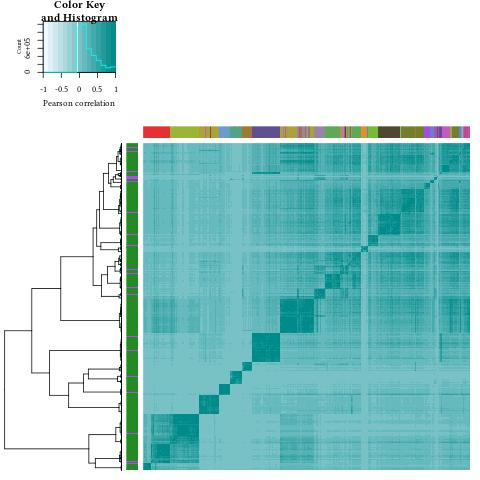
\includegraphics[scale=0.95]{transcriptomics/heatmap23Replicates.jpg}\centering
    \caption[Heatmap including all the replicates of the 23 common tissues
    between Uhlén and GTEx studies]{\label{fig:noMitoRep23T}\textbf{Heatmap
    including all the replicates of the twenty-three common tissues between
    Uhlén et al.\ and GTEx studies.} All protein-coding genes (except the mitochondrial ones)
    at least expressed at 1 \FPKM\ are included. Most samples are clustering by
    their tissue of origin while we can observe than many single replicates may
    cluster less expectedly. Many small mixtures are observed; often they involve
    closely related tissues, \ie\ \tissue{Heart} and \tissue{Skeletal muscle} or
    \tissue{Ovary} and \tissue{Fallopian tube}.}
\end{figure}



\begin{figure}[!htpb]
\centering
\begin{minipage}{\textwidth}
\begin{subfigure}[b]{0.95\textwidth}
\centering
\includegraphics[scale=0.9]%
{transcriptomics/TransPearsonDistributionIdenticalDifferent.pdf}
\caption[Pearson correlation]{\label{fig:distribPearsCorr}\textbf{Pearson
correlation}}
\end{subfigure}

\begin{subfigure}[b]{0.95\textwidth}
\centering
\includegraphics[scale=0.9]%
{transcriptomics/TransSpearmanDistributionIdenticalDifferent.pdf}
\caption[Spearman correlation]{\label{fig:distribSpearCorr}\textbf{Spearman
correlation}}
\end{subfigure}
\caption[Distribution of the correlation of matched and unmatched tissues pairs
across the two working sets.]{\label{fig:distribCorr}%
\textbf{Distribution of the correlation of matched
and unmatched tissues pairs for the two working sets.} The displayed
p-values\footnote{Thresholds above which the $H_0$ hypothesis
is safe to be rejected.\\$H_0$: The correlations of same tissue pairs and
different tissues pairs are similar.} have been computed with
a Welch two-sample t-test.}
\end{minipage}
\end{figure}

\FloatBarrier\
%\clearpage

\section{Overlap of the top high expressed genes between the five datasets}\label{sec:overlapHighExp}

\begin{figure}[!htbp]
\includegraphics[scale=1]{transcriptomics/highExpress4TP.pdf}\centering
\caption[Cumulative shared set of genes ranked by expression across the 5
studies]{\label{fig:highExpress4T}\textbf{Cumulative shared set of genes
ranked by their decreasing order of expression across the five studies.}
Apart from a very small subset for the highest expressed protein coding genes,
the overlap of the gene ranks across the 5 studies is rather small.
The grey line presents the evolution of the ratios for the randomly
permuted data which highlights that there is an underlying structure.}
\end{figure}

\Cref{fig:highExpress4T} shows the ratios of the number of
common \pcgs\ for a given amount of highest expressed \pcgs\
to that very number across the studies and for each tissue.
Among these (cumulative) proportions,
a few present very high value for
a minimal subset of genes (below $10$ \FPKM\ across all the tissues)
which then drop dramatically to finally increase slowly
to reach the expected ratio of $1$ \FPKM{}.
\begin{comment}
as the \pcgs\ set across the studies is identical.
\end{comment}

\begin{figure}[!htbp]
    \includegraphics[scale=0.8]{transcriptomics/highExpress23TP.pdf}\centering
    \caption[Cumulative shared set of genes, sorted by their expression, between
    Uhlen and GTEx]{\label{fig:highExpress23T}\textbf{Cumulative shared set of
    genes, ranked by their decreasing order of expression, between Uhlén et al.\
    and GTEx studies.}
    The highest expressed genes present greater ratios than
    when the 5 studies are considered (see \Cref{fig:highExpress4T}).
    The fewer number of studies considered, which, additionally to be the most
    recent studies, are the ones to comprise greater number of biological
    replicates per tissues may be the sole reasons for the improved results.}
\end{figure}

\Cref{fig:highExpress23T} presents the same kind of ratios,
however, limited to \uhlen\ and \gtex\ only.
Here as well, aside from the expected perfect ratio for the complete set of
\pcgs,
only a tiny subset of the highest expressed genes produce high rates of
highly expressed common genes to the number of considered ranked genes.
These results are quite unsurprising as they involve only two studies.
In addition to increasing the number of overlaps probabilistically,
these two studies are also the two most recent ones
and comprise a higher number of replicates per tissues;
thus the measurements for each gene in each condition are likely more robust.

Comparing the calculated ratios between the real (colour) and
the randomly permuted data (grey)
on \Cref{fig:highExpress4T,fig:highExpress23T}
plainly show that there are common (biological) structures
that are nonfortuitous across studies.
\FloatBarrier\
\section{Variable genes}

\begin{sidewaysfigure}[htpb]
    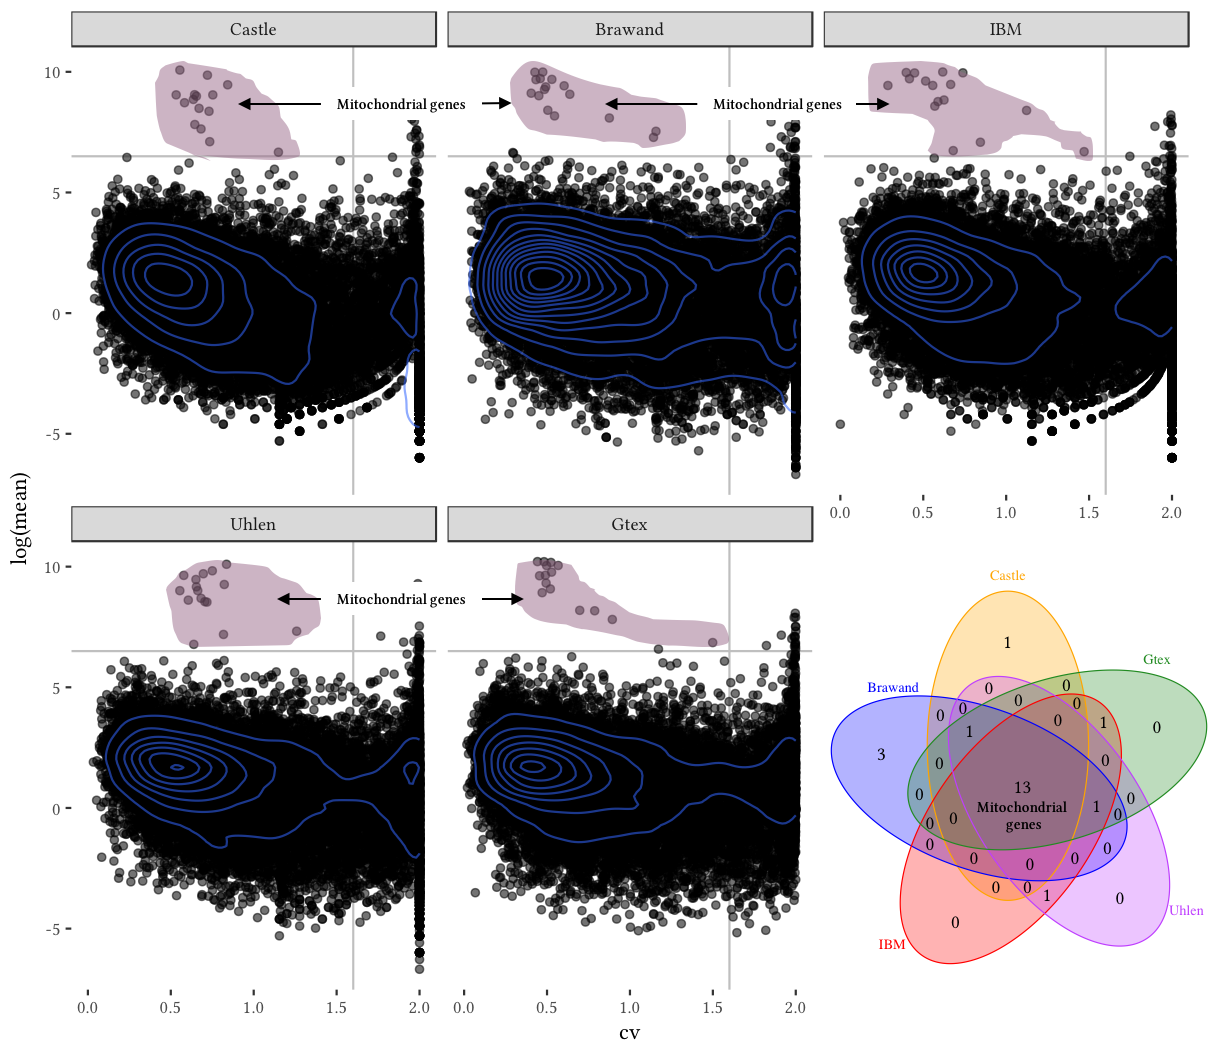
\includegraphics[scale=1]{transcriptomics/MitoVarianceFinale.png}\centering
    \caption[Mean expression of genes compared to their coefficient of variation]%
    {\label{fig:MitoVar}\textbf{Mean expression of genes compared to their
    coefficient of variation.}}
\end{sidewaysfigure}

\begin{figure}[!htpb]
    \includegraphics[scale=0.7]{transcriptomics/Overlap_25p_mostCoeffVariablesgenes.pdf}\centering
    \caption[Overlap of the most variables genes across the 5 studies for the set
    of four common tissues]{\label{fig:vennMostVar4T}\textbf{Overlap of the most
    variable genes across the five studies for the set of the four common tissues.}
    In each study, I rank the \pcgs\ in decreasing order.
    This Venn diagram presents the shared and unique \pcgs\ in the top
    quarter of the most variable genes.
    }
\end{figure}

\minisec{Two-sample test}\label{mini:ttest}
Welch's test~\mycite{Welch1947-rv},
also known as the unequal variances \ttest,
is an adaptation of the Student \ttest{}~\mycite{student_1908}
and it is better fitted for groups that have different variance and sample sizes.
Except in the case of (true) paired data (sampled on the same source),
it gives better or at least equal results than the traditional
Student \ttest~\mycite{Fagerland2012-vl,Derrick2016-mc,Delacre2017-ya}.

Student's two-sample location test (\ie\ \ttest) is a test
where the null hypothesis is defines as the means of the two populations
which have been sampled are equal.
Student's \ttest\ relies on the assumption that the variance of the population is
also equal.



\begin{figure}[!htbp]
    \includegraphics[scale=0.90]%
    {transcriptomics/Heatmap_25p_mostCoeffVariablesgenes_spearman.pdf}\centering
    \vspace{-12mm}
    \caption[Clustering of the four common tissues across the five studies for
    the most common variable genes]%
    {\label{fig:heatmapMost25pVariable}\textbf{Clustering of the four common
    tissues across the five studies for the most common variable genes.}
    The samples cluster by tissue of origin
    rather than by original study.
    Each cluster of tissue presents a different hierarchy of study:
    for \kidney, \uhlen\ sample is closer to the \ibm\ sample,
    while for \testis, \uhlen\ sample is closer to the \gtex\ one.}
\end{figure}

\begin{figure}[!htbp]
    \includegraphics[scale=0.90]%
    {transcriptomics/Reverse_heatmap_25p_mostCoeffVariablesgenes_Spearman.pdf}\centering
    \vspace{-12mm}
    \caption[Clustering of the the four common tissues across the five studies
    (excluding the most common variable genes)]{\label{fig:ReverseheatmapMost25pVariable}%
    \textbf{Clustering of the four common tissues across the five studies
    (excluding the most variable genes).} Apart from the Castle samples,
    the samples cluster by tissue of origin rather than by original study.
    (Note that Pearson correlations give stronger clustering results towards
    the biological origin of the \treps.)}
\end{figure}

\begin{figure}[!htpb]
    \includegraphics[scale=0.8]{transcriptomics/Heatmap_25p_mostCoeffVariablesgenesTheirExpression.pdf}\centering
    \vspace{-4mm}
    \caption[Expression of the most common variable genes]{\label{fig:expressionMostvariableG}
    \textbf{Expression of the most common variable genes.} }
\end{figure}

\begin{figure}[!htbp]
    \includegraphics[scale=0.8]{transcriptomics/MaxSumExpressionHighCVgenes4TStackedHistogram.pdf}\centering
    \vspace{-2mm}
    \caption[Maximum of expression / Sum of expression for the most variable genes]%
    {\label{fig:highestCVhist}\textbf{Ratio of Maximum of expression/Sum of expression
    for the most variable genes (cv≥1.5) in \setOne that are expressed at least
    in two different tissues at 1 FPKM.} The lowest ratio is above $0.79$ and the highest
    ratio is close to 1. This range shows that the most variable genes are
    expressed in one tissue more specifically than the three others as the tissue
    where they are the highest expressed accounts for more than 79\% of the sum
    of expression across the four tissues.}
\end{figure}

\begin{comment}
\begin{figure}[htpb]
    \includegraphics[scale=1]{transcriptomics/mostSpe23TP.pdf}\centering
    \caption[Cumulative shared set of genes, sorted by their specificity, between
Uhlen and GTEx]{\label{fig:mostSpe23T}\textbf{Cumulative shared set of genes
ordered by their decreasing order of specificity to each tissue between \uhlen\
and \gtex.}}
\end{figure}
\end{comment}

\begin{figure}
    \centering
    \begin{subfigure}[b]{\textwidth}
        \centering \includegraphics[width=0.4\textwidth]%
        {transcriptomics/breadthMostVariable/CastleMostVarGenesBreadth.pdf}
        \caption{Castle}
    \end{subfigure}%
~%
    \begin{subfigure}[b]{\textwidth}
        \centering \includegraphics[width=0.4\textwidth]%
        {transcriptomics/breadthMostVariable/BrawandMostVarGenesBreadth.pdf}
        \caption{Brawand}
    \end{subfigure}%

    \begin{subfigure}[b]{\textwidth}
        \centering \includegraphics[width=0.4\textwidth]%
        {transcriptomics/breadthMostVariable/IBMMostVarGenesBreadth.pdf}
        \caption{IBM}
    \end{subfigure}%
~%
    \begin{subfigure}[b]{\textwidth}
        \centering \includegraphics[width=0.4\textwidth]%
        {transcriptomics/breadthMostVariable/UhlenMostVarGenesBreadth.pdf}
        \caption{Uhlen}
    \end{subfigure}%

    \begin{subfigure}[b]{\textwidth}
        \centering \includegraphics[width=0.4\textwidth]%
        {transcriptomics/breadthMostVariable/GtexMostVarGenesBreadth.pdf}
        \caption{GTEx}
    \end{subfigure}%
    \caption[Breadth of expression (≥1 FPKM) for the most variable mRNAs]%
    {\label{fig:mostVarBreadth}%
    \textbf{Breadth of expression (≥1 FPKM) for the most variable mRNAs (cv≥1.5)
    across \setOne.} Most of these \mRNAs\ are expressed only at 1 \FPKM\ or above.}
\end{figure}


\begin{sidewaysfigure}[!htpb]
    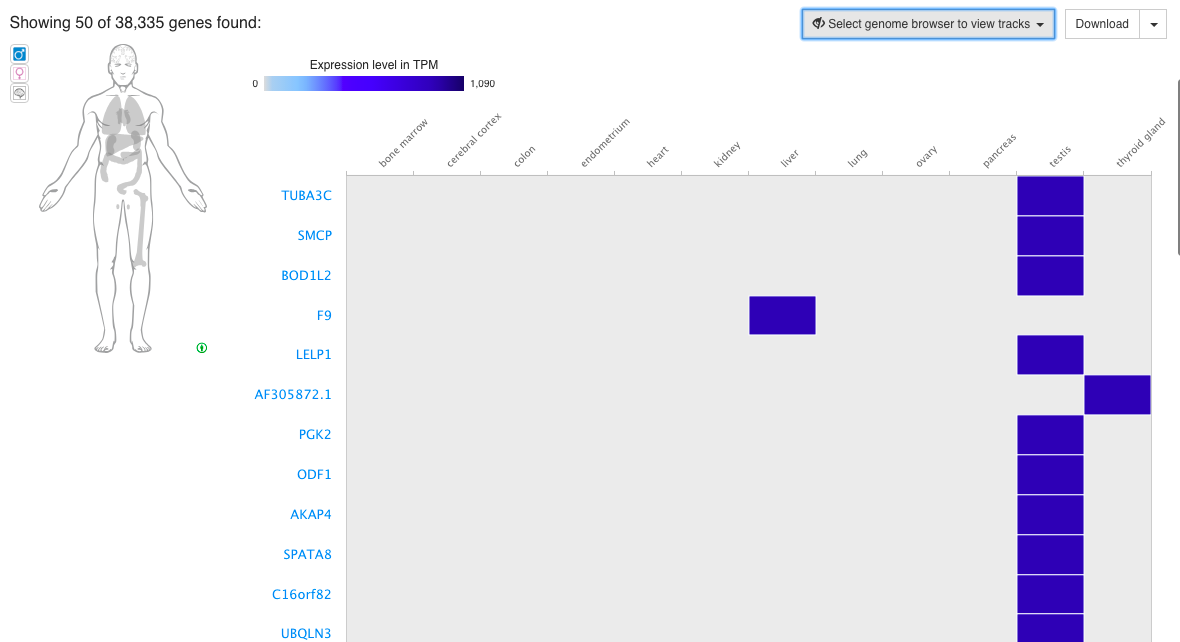
\includegraphics[scale=0.55]{transcriptomics/ebiGxaEx.png}\centering
    \caption[Most specific genes highlighted in EBI gene expression atlas]{\label{fig:gxaEx}%
    \textbf{Most specific genes highlighted in EBI gene expressio atlas.}}
\end{sidewaysfigure}

\FloatBarrier\

\section{Hampel method}\label{sec:hampel}

The Hampel method allows detecting outliers and
it relies on the median and the \gls{MAD} (median absolute deviation)
as robust estimate of the location and spread (instead of the more commonly
used mean and standard deviation). \mycite{Hampel1971,Hampel1974}

\begin{algorithm}[H]
\SetAlgoLined\
\KwData{Expression matrix; Genes as rows and conditions (tissues) as columns}\
\KwIn{threshold: numeric}\
\KwIn{bool: boolean}\
\KwResult{Indicates if a gene presents an \emph{atypical} (outlier) expression
for any condition (as a boolean or a numeric ratio)}
\BlankLine\
\ForEach{Gene g (\ie\ row) of the input matrix}{%
    med=compute median(g)\;
    \tcc{compute the M.A.D.\ (median absolute deviation)}
    mad=median(absolute(g-med))\;
\eIf{!bool}{%
\tcc{Return boolean answer}
newg=absolute(g-med) > threshold*mad\;
}{%
\tcc{Return ratios that can be later sorted}
newg=(absolute(g-med))/mad\;
}
return(newg)\;
}
\caption{Hampel method}\label{algo:hampel}
\end{algorithm}

\subsection{Median}
Median can be found by listing all values from smallest to greatest.\\
If the number of values is odd, the median is the middle value.\\
If the number of values is even, the median is the mean of the two middle values.

\subsection{Median absolute deviation (M.A.D.)}
For a give variable X, M.A.D.\ is defined as follow:

\begin{equation}\label{eq:mad}
    \tag{M.A.D.}
MAD = median(|X_{i}-median(X)|)
\end{equation}


\section{List of the tissues available in TiGER}\label{sec:supplTiger}

Thirty tissues (or equivalent) are available through this database:
\tissue{Bladder}, \tissue{Blood}, \tissue{Bone}, \tissue{Bone marrow},
\tissue{Brain}, \tissue{Cervix}, \tissue{Colon}, \tissue{Eye},
\tissue{Heart}, \tissue{Kidney}, \tissue{Larynx}, \tissue{Liver},
\tissue{Lung}, \tissue{Lymph node}, \tissue{Mammary gland}, \tissue{Muscle},
\tissue{Ovary}, \tissue{Pancreas}, \tissue{Peripheral nervous system},
\tissue{Placenta}, \tissue{Prostate}, \tissue{Skin},
\tissue{Small intestine}, \tissue{Soft tissue}, \tissue{Spleen},
\tissue{Stomach}, \tissue{Testis}, \tissue{Thymus}, \tissue{Tongue} and \tissue{Uterus}.

\begin{comment}
\begin{sidewaystable}[]
\centering
\caption{Shared definition of TIGER's \emph{specific} genes across tissues}
\label{tab:TiGERperTissue}
\begin{tabular}{@{}cccccccccccccccccc@{}}
\toprule
 & Bladder & Brain & Colon & Heart & Kidney & Liver & Lung & Muscle & Ovary &
 Pancreas & Prostate & Skin &
 \begin{tabular}[c]{@{}c@{}}Small\\ intestine\end{tabular}
 & Spleen & Stomach & Testis & Uterus \\
\midrule
Bladder & 138 & 0 & 4 & 2 & 1 & 6 & 1 & 0 & 0 & 0 & 1 & 3 & 1 & 7 & 1 & 6 & 0 \\
Brain & 0 & 282 & 0 & 0 & 0 & 0 & 0 & 0 & 0 & 0 & 0 & 0 & 0 & 0 & 0 & 0 & 0 \\
Colon & 4 & 0 & 154 & 1 & 12 & 3 & 1 & 0 & 1 & 2 & 1 & 1 & 5 & 1 & 12 & 0 & 0 \\
Heart & 2 & 0 & 1 & 167 & 6 & 1 & 0 & 40 & 5 & 0 & 2 & 2 & 3 & 5 & 1 & 0 & 0 \\
Kidney & 1 & 0 & 12 & 6 & 314 & 39 & 0 & 4 & 3 & 3 & 5 & 0 & 0 & 2 & 3 & 5 & 0 \\
Liver & 6 & 0 & 3 & 1 & 39 & 285 & 1 & 7 & 0 & 3 & 1 & 2 & 3 & 14 & 5 & 9 & 0 \\
Lung & 1 & 0 & 1 & 0 & 0 & 1 & 114 & 0 & 0 & 3 & 2 & 0 & 0 & 0 & 2 & 1 & 0 \\
Muscle & 0 & 0 & 0 & 40 & 4 & 7 & 0 & 203 & 1 & 1 & 2 & 1 & 5 & 2 & 0 & 1 & 0 \\
Ovary & 0 & 0 & 1 & 5 & 3 & 0 & 0 & 1 & 110 & 1 & 1 & 0 & 1 & 1 & 5 & 2 & 1 \\
Pancreas & 0 & 0 & 2 & 0 & 3 & 3 & 3 & 1 & 1 & 145 & 0 & 1 & 2 & 0 & 8 & 2 & 0 \\
Prostate & 1 & 0 & 1 & 2 & 5 & 1 & 2 & 2 & 1 & 0 & 127 & 2 & 1 & 1 & 1 & 3 & 0 \\
Skin & 3 & 0 & 1 & 2 & 0 & 2 & 0 & 1 & 0 & 1 & 2 & 143 & 0 & 0 & 0 & 2 & 0 \\
\begin{tabular}[c]{@{}c@{}}Small\\ intestine\end{tabular} & 1 & 0 & 5 & 3 & 0 & 3 & 0 & 5 & 1 & 2 & 1 & 0 & 96 & 3 & 1 & 1 & 0 \\
Spleen & 7 & 0 & 1 & 5 & 2 & 14 & 0 & 2 & 1 & 0 & 1 & 0 & 3 & 97 & 8 & 2 & 0 \\
Stomach & 1 & 0 & 12 & 1 & 3 & 5 & 2 & 0 & 5 & 8 & 1 & 0 & 1 & 8 & 174 & 1 & 1 \\
Testis & 6 & 0 & 0 & 0 & 5 & 9 & 1 & 1 & 2 & 2 & 3 & 2 & 1 & 2 & 1 & 636 & 2 \\
Uterus & 0 & 0 & 0 & 0 & 0 & 0 & 0 & 0 & 1 & 0 & 0 & 0 & 0 & 0 & 1 & 2 & 39 \\
\bottomrule
\end{tabular}
\end{sidewaystable}
\end{comment}


%\clearpage
\section{List of publications based on RNA-Seq and covering at least partially its robustness}\label{sec:TranssCoop}
\begin{flushleft}
\begin{itemize}
    \item\fullcite{seqcmaqc}
%    \item~\fullcite{Rau2014-va}
    \item\fullcite{Santos2015-rj}
    \item\fullcite{Sudmant2015-zt}
    \item\fullcite{Danielsson2015-cn}
    \item\fullcite{Uhlen:2016}
    \item\fullcite{ruvseqComQN}
    \item\fullcite{Wang2017-hc}
\end{itemize}
\end{flushleft}

\section{Complement~to~the~highest~genes~anticorrelations}\label{sec:whyAnticor}

As very few genes are involved,
the slightest changes in their respective order of magnitude
may imply reversed trends.

\begin{table}[!h]
\centering
\caption{Example of gene subsets for a two studies (A and B) for a tissue}
\label{tab:anticorExample}
\begin{tabular}{@{}llllll@{}}
\toprule
 & $Gene_a$ & $Gene_b$ & $Gene_c$ & $Gene_d$ & $Gene_e$ \\
\midrule
Study A, \trep\ $T_1$ ($T^{Study A}_1$) & 1000 & 2000 & 3000 & 4000 & 5000 \\
Study B, \trep\ $T_1$ ($T^{Study B}_1$) & 500 & 2800 & 6000 & 5000 & 4000 \\
\bottomrule
\end{tabular}
\end{table}

For example,
if we consider $T^{Study A}_1$ and $T^{Study B}_1$
for a set of genes ${a, \ldots, e}$ (see \Cref{tab:anticorExample})
and a cut-off at 3,000 \FPKMs,
then the correlation will only involve $Gene_c$, $Gene_d$ and $Gene_e$.
Thus,\\
while $corr_{T^{Study A}_1,T^{Study B}_1}(c,d,e)= -1 $,\\
$corr_{T^{Study A}_1,T^{Study B}_1}(a,b,c,d,e)= 0.6836$

\begin{figure}[!htbp]
    \includegraphics[scale=1]{transcriptomics/AnticorrExample.pdf}\centering
    \caption{Example on how correlation may change to cut-offs}\label{fig:anticorrExample}
\end{figure}
\FloatBarrier\
\section{Uhlén categories}\label{sec:suppUhlen}

\begin{sidewaystable}[]
\centering
\caption{Uhlén et al.\ gene categories for all genes (\ie\ unrestricted to protein-coding genes)}
\label{tab:uhlenCatAllgenes}
\begin{tabular}{@{}ccccccccccc@{}}
\toprule
\multicolumn{2}{c}{\multirow{2}{*}{\begin{tabular}[c]{@{}c@{}}\ens{76}
\\(62,757 gene definitions) \end{tabular}}} &
\multirow{2}{*}{\begin{tabular}[c]{@{}c@{}}\\Not\\detected\end{tabular}} &
\multirow{3}{*}{\begin{tabular}[c]{@{}c@{}}Not expressed\\ at 1 \gls{FPKM}\\
    cut-off\end{tabular}} &
\multicolumn{2}{c}{Mixed expression} &
\multicolumn{2}{c}{Ubiquitous expression} &
\multirow{2}{*}{\begin{tabular}[c]{@{}c@{}}\\Group \\Enhanced\end{tabular}} &
\multirow{2}{*}{\begin{tabular}[c]{@{}c@{}}\\Tissue\\ Enhanced\end{tabular}} &
\multirow{2}{*}{\begin{tabular}[c]{@{}c@{}}\\Tissue\\ Enriched\end{tabular}} \\
\cmidrule(lr){5-8}
\multicolumn{2}{c}{}   &  &  &
    \begin{tabular}[c]{@{}c@{}}Low\\ (\textless\ 10 \gls{FPKM})\end{tabular} &
    \begin{tabular}[c]{@{}c@{}}High\\ (≥ 10 \gls{FPKM})\end{tabular} &
    \begin{tabular}[c]{@{}c@{}}Low\\ (\textless\ 10 \gls{FPKM})\end{tabular} &
    \begin{tabular}[c]{@{}c@{}}High\\ (≥ 10 FPKM)\end{tabular} &  &  &  \\
\midrule
\multicolumn{1}{c}{%
    \multirow{7}{*}{\rotatebox[origin=c]{90}{\parbox[c]{4cm}{\centering Whole
     dataset}}}} &
     Castle & 18,836 & 16,258 & 19,079 & 1,203  &
     1,456  & 703  & 77  & 8,319  & 3,896 \\
     \multicolumn{1}{c}{} & Brawand & 18,278 & 20,173 &
     15,254 & 2,057  & 1,873 & 977   & 0  &
     6,180  & 5,442 \\
     \multicolumn{1}{c}{} & IBM & 14,494 & 20,858  &
     16,633  & 1,582  & 1,194 & 926  & 733 &
     10,042  & 4,453  \\
     \multicolumn{1}{c}{} & Uhlen & 17,345 & 16,548 &
     15,372 & 1,351  & 467 & 419  & 4,615  &
     10,644 & 5,498  \\
     \multicolumn{1}{c}{} & Gtex  & 5,755  & 25,138  &
     17,172  & 1,464 & 775  & 713  & 7,164  &
     10,032  & 5,117 \\ \cmidrule(l){2-11}
     \multicolumn{1}{c}{} & Consensus & 5,747 & 4,231  &
     4,121  & 230  & 33  & 166  & 0  & 1,073  &
     \begin{tabular}[c]{@{}c@{}}531 $[$518$]$\end{tabular} \\
\midrule
\multirow{7}{*}{\rotatebox[origin=c]{90}{\parbox[c]{3cm}{\centering Common\\
4 tissues\\ Working datasets}}} &
Castle & 43,921 & 3,267 & 14,850 & 1,735 &
3,267 & 1,181 & --- & --- & 4,645 \\
& Brawand & 44,479  & 3,193  & 13,975 & 2,541
& 3,193  & 1,282 & --- & --- & 7,002  \\
& IBM & 48,263  & 3,262 & 13,672 & 2,160 &
3,262  & 1,299  & --- & --- & 5,242  \\
& Uhlen & 45,412 & 3,146 & 14,332 & 2,546 &
3,146 & 1,213  & --- & --- & 7,665  \\
& Gtex & 57,002 & 4,516 & 16,652  & 2,771 &
4,516  & 1,459  & --- & --- & 8,155  \\
\cmidrule(l){2-11}
& Consensus & 9,655 & 557 & 4,366 & 675 &
557  & 448 & --- & --- & 1,960  \\
\\ \midrule
\multirow{3}{*}{\rotatebox[origin=c]{90}{\parbox[c]{1.7cm}{\centering Common\\ 23
tissues\\ Working datasets}}} & Uhlen & 17,345  & 27,575  &
14,981 & 1,427 & 611  & 440 & 2,203 & 11,252 & 5,678 \\
& Gtex & 5,755 & 38,988 & 16,982  & 1,909 & 2,122  & 1,021 & 1,746 & 11,236
& 5,971 \\
\cmidrule(l){2-11}
& Consensus & 5,755 & 27,149 & 12,250 & 973 &
433 & 430 & 797 & 8,030 & 4,281 \\
\bottomrule
\end{tabular}
\end{sidewaystable}


